\documentclass[a4paper,12pt]{paper}

\usepackage{mycommands}

% Worked-example layout: boxed problem statement followed by a solution.
\newcounter{example}
\renewenvironment{example}[1]{%  % the paper class already defines "example"
  \refstepcounter{example}%
  \begin{mdframed}[linewidth=1pt,innertopmargin=6pt,innerbottommargin=6pt]%
  \noindent\textbf{Example \theexample: #1.}\ }{%
  \end{mdframed}}
\newenvironment{solution}{\par\noindent\textbf{Solution.}\ }{\par\medskip}

\title{Worked examples for Lecture 15: Plane wave propagation}
\author{David Al-Attar \\ Michaelmas Term, \the\year}

\begin{document}

\maketitle

\noindent These examples accompany Lecture~15. They are intended as practice in the concrete
calculations that underlie the lecture, and are less demanding than the questions on the
problem sets. Throughout, $\rho$ is the referential density, $A_{ijkl}$ the elastic tensor,
$\bm{\Gamma}(\hat{\mathbf{p}})$ the Christoffel matrix for a unit propagation direction
$\hat{\mathbf{p}}$, and the phase speeds $c$ and polarisation vectors $\mathbf{a}$ satisfy the
Christoffel equation $\bm{\Gamma}(\hat{\mathbf{p}})\mathbf{a}=c^{2}\mathbf{a}$. Numerical results
were checked with the scripts in the \texttt{python} directory.

%------------------------------------------------------------------------------
\begin{example}{P- and S-waves with numbers}
At a depth of $100\,\mathrm{km}$ the Preliminary Reference Earth Model (PREM) has, to three
significant figures, $\rho=3.38\times10^{3}\,\mathrm{kg\,m^{-3}}$, bulk modulus
$\kappa=1.30\times10^{11}\,\mathrm{Pa}$ and shear modulus $\mu=6.80\times10^{10}\,\mathrm{Pa}$.
Compute the Lamé parameter $\lambda$, the P- and S-wave speeds $\alpha$ and $\beta$, the ratio
$\alpha/\beta$, and Poisson's ratio $\sigma=\lambda/[2(\lambda+\mu)]$. Show that $\alpha/\beta$
depends on the elastic moduli only through $\sigma$, and check that
$\alpha/\beta=\sqrt{3}$ for a Poisson solid, for which $\lambda=\mu$.
\end{example}

\begin{solution}
We recall from the lecture that the bulk modulus of an isotropic solid is $\kappa=\lambda+\tfrac{2}{3}\mu$, and hence
\begin{equation}
\lambda=\kappa-\tfrac{2}{3}\mu=1.30\times10^{11}-0.453\times10^{11}=8.47\times10^{10}\,\mathrm{Pa}.
\label{eq:1}
\end{equation}
The P- and S-wave speeds follow from the solution of the Christoffel equation for an isotropic
medium. It is convenient to write the P-wave modulus as
$\lambda+2\mu=\kappa+\tfrac{4}{3}\mu=2.21\times10^{11}\,\mathrm{Pa}$, so that
\begin{equation}
\begin{split}
\alpha&=\sqrt{\frac{\lambda+2\mu}{\rho}}=\sqrt{\frac{2.207\times10^{11}}{3.38\times10^{3}}}\,\mathrm{m\,s^{-1}}
=8.08\,\mathrm{km\,s^{-1}},\\
\beta&=\sqrt{\frac{\mu}{\rho}}=\sqrt{\frac{6.80\times10^{10}}{3.38\times10^{3}}}\,\mathrm{m\,s^{-1}}
=4.49\,\mathrm{km\,s^{-1}}.
\end{split}
\label{eq:2}
\end{equation}
Note that with all quantities in SI units the speeds come out in $\mathrm{m\,s^{-1}}$; a
common slip is to mix $\mathrm{GPa}$ with $\mathrm{kg\,m^{-3}}$ and obtain speeds that are
wrong by a factor of $\sqrt{10^{9}}$. The ratio of the speeds and Poisson's ratio are
\begin{equation}
\frac{\alpha}{\beta}=\frac{8.080}{4.485}=1.80,\quad
\sigma=\frac{\lambda}{2(\lambda+\mu)}=\frac{8.47}{2\times15.27}=0.277.
\label{eq:3}
\end{equation}

To relate the two, we note that the definition of $\sigma$ can be inverted to give
\begin{equation}
\frac{\lambda}{\mu}=\frac{2\sigma}{1-2\sigma},
\label{eq:4}
\end{equation}
and hence
\begin{equation}
\frac{\alpha^{2}}{\beta^{2}}=\frac{\lambda+2\mu}{\mu}=2+\frac{\lambda}{\mu}=\frac{2(1-\sigma)}{1-2\sigma}.
\label{eq:5}
\end{equation}
The ratio of the wave speeds is, therefore, a function of Poisson's ratio alone, and conversely
a measurement of $\alpha/\beta$ determines $\sigma$ without knowledge of the density. With
$\sigma=0.277$ eq.~(\ref{eq:5}) gives $\alpha/\beta=1.80$, in agreement with eq.~(\ref{eq:3}).
For a Poisson solid $\lambda=\mu$ gives $\sigma=1/4$, and then
$\alpha^{2}/\beta^{2}=2\times\tfrac{3}{4}/\tfrac{1}{2}=3$, so that $\alpha/\beta=\sqrt{3}=1.73$.

The values in PREM are close to, but slightly above, those of a Poisson solid; a value of
$\alpha/\beta$ between $1.7$ and $1.8$ is typical of the crust and mantle, which is why the
Poisson solid is so often used as a rough model in seismology. It is worth remembering that in
practice the logic runs the other way from this example: seismology measures $\alpha$ and
$\beta$, and the moduli in PREM are inferred from them together with the density.
\end{solution}

%------------------------------------------------------------------------------
\begin{example}{The Christoffel matrix in a cubic crystal}
A crystal with cubic symmetry has an elastic tensor of the form
\begin{equation}
A_{ijkl}=c_{12}\,\delta_{ij}\delta_{kl}+c_{44}(\delta_{ik}\delta_{jl}+\delta_{il}\delta_{jk})
+(c_{11}-c_{12}-2c_{44})\sum_{n=1}^{3}\delta_{in}\delta_{jn}\delta_{kn}\delta_{ln},
\label{eq:6}
\end{equation}
where $c_{11}$, $c_{12}$ and $c_{44}$ are the three independent elastic constants in Voigt's
notation and the co-ordinate axes are aligned with the crystal axes. Take the round values
$c_{11}=320\,\mathrm{GPa}$, $c_{12}=70\,\mathrm{GPa}$, $c_{44}=80\,\mathrm{GPa}$ and
$\rho=3300\,\mathrm{kg\,m^{-3}}$, which are of the magnitude found for olivine (though olivine
itself is orthorhombic rather than cubic). Obtain the Christoffel matrix for a general unit
vector $\hat{\mathbf{p}}$, and find the phase speeds and polarisation vectors for propagation
along the $[100]$, $[110]$ and $[111]$ directions, i.e.\ for $\hat{\mathbf{p}}$ proportional to
$(1,0,0)$, $(1,1,0)$ and $(1,1,1)$. For what relation between the constants is the material
isotropic?
\end{example}

\begin{solution}
Writing $d=c_{11}-c_{12}-2c_{44}$ for the coefficient of the last term in eq.~(\ref{eq:6}), and
contracting the elastic tensor with $\hat{p}_{j}\hat{p}_{l}$ term by term, we find
\begin{equation}
\rho\,\Gamma_{ik}(\hat{\mathbf{p}})=A_{ijkl}\hat{p}_{j}\hat{p}_{l}
=c_{12}\hat{p}_{i}\hat{p}_{k}+c_{44}(\delta_{ik}\hat{p}_{j}\hat{p}_{j}+\hat{p}_{i}\hat{p}_{k})
+d\sum_{n=1}^{3}\delta_{in}\delta_{kn}\hat{p}_{n}^{2},
\label{eq:7}
\end{equation}
where in the last term the sum over $j$ and $l$ has collapsed onto $j=l=n$. Since
$\hat{p}_{j}\hat{p}_{j}=1$, this can be written in matrix form as
\begin{equation}
\rho\,\bm{\Gamma}(\hat{\mathbf{p}})=(c_{12}+c_{44})\,\hat{\mathbf{p}}\hat{\mathbf{p}}^{T}+c_{44}\mathbf{I}
+d\,\mathrm{diag}(\hat{p}_{1}^{2},\hat{p}_{2}^{2},\hat{p}_{3}^{2}).
\label{eq:8}
\end{equation}
The first two terms are exactly the isotropic Christoffel matrix of the lecture with
$\lambda=c_{12}$ and $\mu=c_{44}$, and the third term, which is not invariant under rotations
because it singles out the co-ordinate axes, carries all of the anisotropy. The material is
therefore isotropic if and only if $d=0$, i.e.\ $c_{11}-c_{12}=2c_{44}$, in which case
$c_{11}=\lambda+2\mu$ as it should. For our numbers $d=320-70-160=90\,\mathrm{GPa}$, and the
ratio $2c_{44}/(c_{11}-c_{12})=0.64$, which would be unity for an isotropic material, indicates a
strongly anisotropic crystal.

\emph{Propagation along $[100]$.} With $\hat{\mathbf{p}}=(1,0,0)$ the matrix
$\hat{\mathbf{p}}\hat{\mathbf{p}}^{T}$ and the diagonal term are both non-zero only in the
$(1,1)$ entry, so that
\begin{equation}
\rho\,\bm{\Gamma}=\mathrm{diag}(c_{12}+2c_{44}+d,\;c_{44},\;c_{44})=\mathrm{diag}(c_{11},\;c_{44},\;c_{44}).
\label{eq:9}
\end{equation}
The eigenvectors are the co-ordinate axes: a longitudinal wave polarised along
$\hat{\mathbf{e}}_{1}=\hat{\mathbf{p}}$ with $\rho c^{2}=c_{11}$, and a two-fold degenerate
transverse wave with $\rho c^{2}=c_{44}$ whose polarisation can be any vector in the
$(\hat{\mathbf{e}}_{2},\hat{\mathbf{e}}_{3})$-plane. Numerically
$c=\sqrt{320\times10^{9}/3300}=9.85\,\mathrm{km\,s^{-1}}$ and
$c=\sqrt{80\times10^{9}/3300}=4.92\,\mathrm{km\,s^{-1}}$.

\emph{Propagation along $[110]$.} With $\hat{\mathbf{p}}=(1,1,0)/\sqrt{2}$ we have
$\hat{p}_{1}^{2}=\hat{p}_{2}^{2}=\tfrac{1}{2}$, $\hat{p}_{3}=0$, and eq.~(\ref{eq:8}) gives
\begin{equation}
\rho\,\bm{\Gamma}=\frac{c_{12}+c_{44}}{2}\begin{pmatrix}1&1&0\\1&1&0\\0&0&0\end{pmatrix}
+c_{44}\mathbf{I}+\frac{d}{2}\begin{pmatrix}1&0&0\\0&1&0\\0&0&0\end{pmatrix}.
\label{eq:10}
\end{equation}
Rather than expanding the characteristic polynomial we guess the eigenvectors from the structure
of the matrix, as was done for the isotropic case in the lecture. The vector $(1,1,0)/\sqrt{2}$
is an eigenvector of the first matrix with eigenvalue $c_{12}+c_{44}$ and of the third with
eigenvalue $d/2$; the vector $(1,-1,0)/\sqrt{2}$ is annihilated by the first matrix and is an
eigenvector of the third with eigenvalue $d/2$; and $(0,0,1)$ is annihilated by both. Hence
\begin{equation}
\begin{split}
\mathbf{a}=\tfrac{1}{\sqrt{2}}(1,1,0):&\quad \rho c^{2}=c_{12}+2c_{44}+\tfrac{1}{2}d=\tfrac{1}{2}(c_{11}+c_{12}+2c_{44})=275\,\mathrm{GPa},\\
\mathbf{a}=\tfrac{1}{\sqrt{2}}(1,-1,0):&\quad \rho c^{2}=c_{44}+\tfrac{1}{2}d=\tfrac{1}{2}(c_{11}-c_{12})=125\,\mathrm{GPa},\\
\mathbf{a}=(0,0,1):&\quad \rho c^{2}=c_{44}=80\,\mathrm{GPa},
\end{split}
\label{eq:11}
\end{equation}
giving phase speeds of $9.13$, $6.15$ and $4.92\,\mathrm{km\,s^{-1}}$ respectively. The first
wave is longitudinal and the other two transverse, but the two transverse waves now have
different speeds: this is the shear wave splitting discussed at the end of the lecture, and here
it is far from slight, the two S-wave speeds differing by some $25\%$. The polarisation of the
faster S-wave lies in the $(1,2)$-plane, that of the slower one along the third crystal axis.

\emph{Propagation along $[111]$.} With $\hat{\mathbf{p}}=(1,1,1)/\sqrt{3}$ all three
$\hat{p}_{n}^{2}$ equal $\tfrac{1}{3}$, so that the anisotropic term is proportional to the
identity and
\begin{equation}
\rho\,\bm{\Gamma}=(c_{12}+c_{44})\,\hat{\mathbf{p}}\hat{\mathbf{p}}^{T}+\left(c_{44}+\tfrac{1}{3}d\right)\mathbf{I}.
\label{eq:12}
\end{equation}
This has the same form as the isotropic Christoffel matrix, and so can be solved in the same
way: $\hat{\mathbf{p}}$ is an eigenvector, and so is any vector orthogonal to it,
\begin{equation}
\begin{split}
\mathbf{a}=\hat{\mathbf{p}}:&\quad \rho c^{2}=c_{12}+2c_{44}+\tfrac{1}{3}d=\tfrac{1}{3}(c_{11}+2c_{12}+4c_{44})=260\,\mathrm{GPa},\\
\mathbf{a}\perp\hat{\mathbf{p}}:&\quad \rho c^{2}=c_{44}+\tfrac{1}{3}d=\tfrac{1}{3}(c_{11}-c_{12}+c_{44})=110\,\mathrm{GPa},
\end{split}
\label{eq:13}
\end{equation}
with phase speeds $8.88\,\mathrm{km\,s^{-1}}$ and (two-fold degenerate)
$5.77\,\mathrm{km\,s^{-1}}$. All of these eigenvalues were confirmed with a numerical
eigen-decomposition of eq.~(\ref{eq:8}).

Two features are worth noting. First, along the high-symmetry directions $[100]$, $[110]$ and
$[111]$ the waves are purely longitudinal or purely transverse; in a general direction the
eigenvectors of eq.~(\ref{eq:8}) are neither parallel nor perpendicular to $\hat{\mathbf{p}}$,
which is why one speaks of quasi P- and quasi S-waves. Second, the S-wave degeneracy is not
split along $[111]$ even though the crystal is anisotropic: the $[111]$ direction is a three-fold
symmetry axis of the cube, and a symmetric $2\times2$ matrix acting in the plane transverse to
such an axis that is invariant under rotations by $120^{\circ}$ must be a multiple of the
identity. Degeneracies in the slowness surface are thus often dictated by symmetry.
\end{solution}

%------------------------------------------------------------------------------
\begin{example}{The SH sheet of the slowness surface in a transversely isotropic medium}
A transversely isotropic medium with symmetry axis $\hat{\bm{\nu}}$ has elastic tensor
\begin{equation}
\begin{split}
A_{ijkl}=\;&\lambda\delta_{ij}\delta_{kl}+\mu(\delta_{ik}\delta_{jl}+\delta_{il}\delta_{kj})
+8\gamma\hat{\nu}_{i}\hat{\nu}_{j}\hat{\nu}_{k}\hat{\nu}_{l}
+4\xi(\hat{\nu}_{i}\hat{\nu}_{j}\delta_{kl}+\delta_{ij}\hat{\nu}_{k}\hat{\nu}_{l})\\
&-\zeta(\hat{\nu}_{i}\hat{\nu}_{k}\delta_{jl}+\hat{\nu}_{j}\hat{\nu}_{k}\delta_{il}
+\hat{\nu}_{j}\hat{\nu}_{l}\delta_{ik}+\hat{\nu}_{i}\hat{\nu}_{l}\delta_{jk}),
\end{split}
\label{eq:14}
\end{equation}
as in Lecture~13 and the first problem set. Take $\hat{\bm{\nu}}=\hat{\mathbf{e}}_{3}$ and
$\hat{\mathbf{p}}=(\sin\theta,0,\cos\theta)$. Show that $\hat{\mathbf{e}}_{2}$ is an exact
eigenvector of $\bm{\Gamma}(\hat{\mathbf{p}})$ for every $\theta$, and find the corresponding
phase speed. Show that the associated sheet of the slowness surface is an ellipsoid of
revolution, and compare the exact phase speed with the prediction of first-order degenerate
perturbation theory. Illustrate the result for the sample values
$\rho=3300\,\mathrm{kg\,m^{-3}}$, $\lambda=80$, $\mu=70$, $\gamma=2$, $\xi=1$ and
$\zeta=8\,\mathrm{GPa}$.
\end{example}

\begin{solution}
We first form the Christoffel matrix for a general direction. Contracting each term of
eq.~(\ref{eq:14}) with $\hat{p}_{j}\hat{p}_{l}$, and writing
$\hat{\bm{\nu}}\cdot\hat{\mathbf{p}}=\cos\theta$, we obtain
\begin{equation}
\begin{split}
\rho\,\Gamma_{ik}(\hat{\mathbf{p}})=\;&(\lambda+\mu)\hat{p}_{i}\hat{p}_{k}+\mu\delta_{ik}
+8\gamma\cos^{2}\theta\,\hat{\nu}_{i}\hat{\nu}_{k}
+4\xi\cos\theta\,(\hat{\nu}_{i}\hat{p}_{k}+\hat{p}_{i}\hat{\nu}_{k})\\
&-\zeta[\hat{\nu}_{i}\hat{\nu}_{k}+\cos\theta\,(\hat{\nu}_{i}\hat{p}_{k}+\hat{p}_{i}\hat{\nu}_{k})+\cos^{2}\theta\,\delta_{ik}].
\end{split}
\label{eq:15}
\end{equation}
Now let this matrix act on $\hat{\mathbf{e}}_{2}$. Every term in eq.~(\ref{eq:15}) other than
the two proportional to $\delta_{ik}$ contains a factor of either $\hat{p}_{k}$ or
$\hat{\nu}_{k}$, and both $\hat{p}_{k}\hat{e}_{2k}=0$ and $\hat{\nu}_{k}\hat{e}_{2k}=0$ because
$\hat{\mathbf{e}}_{2}$ is orthogonal to the plane containing the propagation direction and
the symmetry axis. Hence
\begin{equation}
\bm{\Gamma}(\hat{\mathbf{p}})\hat{\mathbf{e}}_{2}=\frac{\mu-\zeta\cos^{2}\theta}{\rho}\,\hat{\mathbf{e}}_{2},
\label{eq:16}
\end{equation}
so that $\hat{\mathbf{e}}_{2}$ is an exact eigenvector for all $\theta$, with squared phase speed
\begin{equation}
c_{\mathrm{SH}}^{2}=\frac{\mu-\zeta\cos^{2}\theta}{\rho}=\frac{\mu\sin^{2}\theta+(\mu-\zeta)\cos^{2}\theta}{\rho}.
\label{eq:17}
\end{equation}
This wave is transverse and polarised horizontally (if we think of $\hat{\bm{\nu}}$ as vertical),
and so is called the SH wave. Its speed varies from $\sqrt{\mu/\rho}$ for horizontal propagation to
$\sqrt{(\mu-\zeta)/\rho}$ along the axis, and a positive squared speed along the axis requires
$\mu>\zeta$. Because eigenvectors of a symmetric matrix with distinct eigenvalues are
orthogonal, the remaining two polarisation vectors lie in the $(\hat{\mathbf{e}}_{1},\hat{\mathbf{e}}_{3})$-plane spanned by $\hat{\mathbf{p}}$ and $\hat{\bm{\nu}}$; they are the quasi P- and
quasi SV-waves, whose speeds require the solution of a genuine $2\times2$ eigenvalue problem
and are not in general given by such a simple formula. Nothing in the argument depended on
$\hat{\mathbf{p}}$ lying in the $(1,3)$-plane: by the rotational symmetry about
$\hat{\bm{\nu}}$, for any $\hat{\mathbf{p}}$ making an angle $\theta$ with the axis the vector
$\hat{\bm{\nu}}\times\hat{\mathbf{p}}/\sin\theta$ is an exact eigenvector with the eigenvalue in
eq.~(\ref{eq:17}).

\emph{The slowness sheet.} The slowness vector of the SH wave is
$\mathbf{p}=\hat{\mathbf{p}}/c_{\mathrm{SH}}$, so that
$\|\mathbf{p}\|^{2}=\rho/(\mu-\zeta\cos^{2}\theta)$ and $p_{3}=\|\mathbf{p}\|\cos\theta$. Multiplying
out,
\begin{equation}
\mu\|\mathbf{p}\|^{2}-\zeta p_{3}^{2}=\rho\quad\Longleftrightarrow\quad
\mu(p_{1}^{2}+p_{2}^{2})+(\mu-\zeta)p_{3}^{2}=\rho,
\label{eq:18}
\end{equation}
which is an ellipsoid of revolution about the symmetry axis with equatorial semi-axis
$\sqrt{\rho/\mu}$ and polar semi-axis $\sqrt{\rho/(\mu-\zeta)}$. For $\zeta>0$ the sheet is
prolate, the slowness being largest, and the speed smallest, along the axis. That one sheet of
the slowness surface of a transversely isotropic medium is exactly an ellipsoid is a
well-known special property; the quasi-P and quasi-SV sheets are quartic surfaces.

\begin{figure}[ht]
\centering
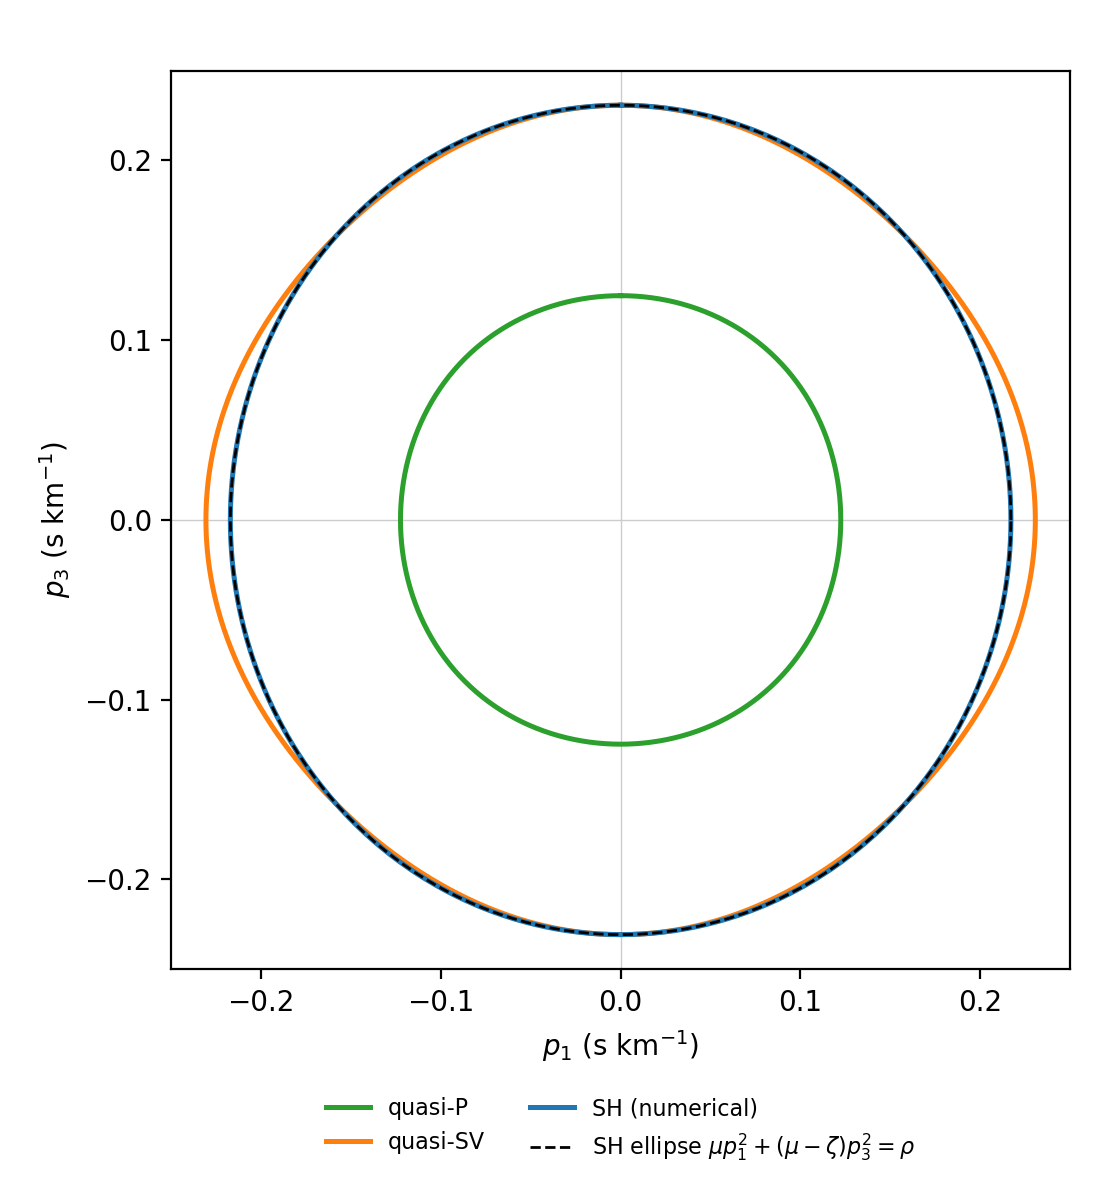
\includegraphics[width=0.7\textwidth]{figures_ex/ex4_slowness_TI.png}
\caption{Section through the slowness surface in the $(p_{1},p_{3})$-plane for the sample
transversely isotropic medium of Example~3, with the symmetry axis vertical. The three sheets
were obtained by numerical diagonalisation of the Christoffel matrix and are labelled by their
polarisation; the dashed curve is the ellipse of eq.~(\ref{eq:18}), on which the numerical SH
sheet lies to machine precision. The SH and quasi-SV sheets touch on the symmetry axis, where
the two S-waves are degenerate, and cross at oblique angles.}
\label{fig:1}
\end{figure}

\emph{Comparison with perturbation theory.} Treating the terms in $\gamma$, $\xi$ and $\zeta$
as the perturbation $\delta\bm{\Gamma}$, with the isotropic part having $\beta^{2}=\mu/\rho$, the
degenerate perturbation theory of the lecture asks us to diagonalise
$\hat{\mathbf{t}}_{a}\cdot\delta\bm{\Gamma}(\hat{\mathbf{p}})\hat{\mathbf{t}}_{b}$ on the plane
orthogonal to $\hat{\mathbf{p}}$. Taking $\hat{\mathbf{t}}_{2}=\hat{\mathbf{e}}_{2}$ and
$\hat{\mathbf{t}}_{1}=\hat{\mathbf{e}}_{2}\times\hat{\mathbf{p}}=(\cos\theta,0,-\sin\theta)$,
eq.~(\ref{eq:16}) shows that $\delta\bm{\Gamma}\hat{\mathbf{e}}_{2}=-(\zeta\cos^{2}\theta/\rho)\hat{\mathbf{e}}_{2}$, and hence
\begin{equation}
\hat{\mathbf{t}}_{1}\cdot\delta\bm{\Gamma}(\hat{\mathbf{p}})\hat{\mathbf{t}}_{2}=0,\quad
\hat{\mathbf{t}}_{2}\cdot\delta\bm{\Gamma}(\hat{\mathbf{p}})\hat{\mathbf{t}}_{2}=-\frac{\zeta\cos^{2}\theta}{\rho}.
\label{eq:19}
\end{equation}
The $2\times2$ matrix is diagonal in this basis, so $\hat{\mathbf{e}}_{2}$ is one of the
zeroth-order polarisations (as it must be, being an exact eigenvector), and the first-order
speed perturbation of the SH wave is
\begin{equation}
\delta\beta_{\mathrm{SH}}=\frac{1}{2\beta}\,\hat{\mathbf{e}}_{2}\cdot\delta\bm{\Gamma}(\hat{\mathbf{p}})\hat{\mathbf{e}}_{2}
=-\frac{\zeta\cos^{2}\theta}{2\rho\beta}=-\frac{\zeta}{2\mu}\beta\cos^{2}\theta.
\label{eq:20}
\end{equation}
The exact result, eq.~(\ref{eq:17}), can be written
\begin{equation}
c_{\mathrm{SH}}=\beta\sqrt{1-\frac{\zeta}{\mu}\cos^{2}\theta}
=\beta\left[1-\frac{\zeta}{2\mu}\cos^{2}\theta-\frac{\zeta^{2}}{8\mu^{2}}\cos^{4}\theta-\cdots\right],
\label{eq:21}
\end{equation}
which agrees with $\beta+\delta\beta_{\mathrm{SH}}$ to first order in $\zeta/\mu$, the error
being of second order as it should be. The perturbation theory gives the eigenvalue $c^{2}$
exactly here; the only approximation is the linearisation of the square root.


For the sample values the SH speed is $4.61\,\mathrm{km\,s^{-1}}$ horizontally and
$4.33\,\mathrm{km\,s^{-1}}$ along the axis, and with $\zeta/\mu=0.114$ the first-order
formula is in error by at most $8\,\mathrm{m\,s^{-1}}$, or $0.2\%$. Fig.~\ref{fig:1} shows
the section of the slowness surface through the $(p_{1},p_{3})$-plane. Along the axis
($\theta=0$) the SH and quasi-SV sheets touch, since eq.~(\ref{eq:15}) shows that
$\bm{\Gamma}(\hat{\bm{\nu}})$ acts as $(\mu-\zeta)/\rho$ times the identity on the plane
orthogonal to $\hat{\bm{\nu}}$: the two S-waves are degenerate along a symmetry axis, exactly
as along $[111]$ in the cubic crystal.
\end{solution}

%------------------------------------------------------------------------------
\begin{example}{First-order perturbation theory checked against exact results}
Write the elastic tensor of the cubic crystal of Example~2 as
$A_{ijkl}=c_{12}\delta_{ij}\delta_{kl}+c_{44}(\delta_{ik}\delta_{jl}+\delta_{il}\delta_{jk})+s\,\delta A_{ijkl}$
with
\begin{equation}
\delta A_{ijkl}=d\sum_{n=1}^{3}\delta_{in}\delta_{jn}\delta_{kn}\delta_{ln},\quad d=c_{11}-c_{12}-2c_{44},
\label{eq:22}
\end{equation}
so that $s=0$ is an isotropic medium with $\lambda=c_{12}$, $\mu=c_{44}$, and $s=1$ is the
crystal itself. (a)~Obtain $\delta\bm{\Gamma}(\hat{\mathbf{p}})$ and the first-order quasi-P
speed perturbation $\delta\alpha$ for a general direction. (b)~For $\hat{\mathbf{p}}$ along
$[110]$ compare $\alpha+\delta\alpha$ with the exact speed found in Example~2, and account for
the discrepancy. (c)~Solve the $2\times2$ degenerate problem for the quasi S-waves along
$[110]$ and show that it reproduces the exact splitting between $\rho c^{2}=\tfrac{1}{2}(c_{11}-c_{12})$ and
$\rho c^{2}=c_{44}$. (d)~For the general direction $\hat{\mathbf{p}}=(2,3,6)/7$ compare the
three first-order eigenvalues with the exact ones, computed numerically, for $s=1$,
$\tfrac{1}{2}$ and $\tfrac{1}{4}$, and hence exhibit the order of the error.
\end{example}

\begin{solution}
(a)~The unperturbed medium has $\alpha^{2}=(c_{12}+2c_{44})/\rho$ and $\beta^{2}=c_{44}/\rho$,
which for the numbers of Example~2 give $\alpha=8.35\,\mathrm{km\,s^{-1}}$ and
$\beta=4.92\,\mathrm{km\,s^{-1}}$. From eq.~(\ref{eq:8}), or directly from the definition
$\delta\Gamma_{ik}=\rho^{-1}\delta A_{ijkl}\hat{p}_{j}\hat{p}_{l}$,
\begin{equation}
\rho\,\delta\bm{\Gamma}(\hat{\mathbf{p}})=d\,\mathrm{diag}(\hat{p}_{1}^{2},\hat{p}_{2}^{2},\hat{p}_{3}^{2}).
\label{eq:23}
\end{equation}
The non-degenerate first-order formula of the lecture then gives, for the quasi P-wave,
\begin{equation}
\delta\alpha=\frac{1}{2\alpha}\hat{\mathbf{p}}\cdot\delta\bm{\Gamma}(\hat{\mathbf{p}})\hat{\mathbf{p}}
=\frac{d}{2\rho\alpha}\left(\hat{p}_{1}^{4}+\hat{p}_{2}^{4}+\hat{p}_{3}^{4}\right).
\label{eq:24}
\end{equation}
Since $\sum_{n}\hat{p}_{n}^{4}$ ranges from $\tfrac{1}{3}$ (along $[111]$) to $1$ (along a cube
axis), the quasi-P speed varies by an amount of order $d/(3\rho\alpha)$ with direction; for
$d>0$ the fastest direction is a cube axis and the slowest is a body diagonal, in agreement with the exact
results of Example~2.

(b)~Along $[110]$ we have $\hat{p}_{1}^{2}=\hat{p}_{2}^{2}=\tfrac{1}{2}$ and $\hat{p}_{3}=0$,
so that $\sum_{n}\hat{p}_{n}^{4}=\tfrac{1}{2}$ and
\begin{equation}
\delta\alpha=\frac{d}{4\rho\alpha}=\frac{90\times10^{9}}{4\times3300\times8348}\,\mathrm{m\,s^{-1}}=0.817\,\mathrm{km\,s^{-1}},
\quad \alpha+s\,\delta\alpha\big|_{s=1}=9.17\,\mathrm{km\,s^{-1}}.
\label{eq:25}
\end{equation}
The exact speed from Example~2 is $\sqrt{275\times10^{9}/3300}=9.13\,\mathrm{km\,s^{-1}}$, so
the first-order result is too large by $37\,\mathrm{m\,s^{-1}}$, or $0.4\%$. To see where this
comes from, note that along $[110]$ the matrix $\rho\,\delta\bm{\Gamma}=\tfrac{1}{2}d\,\mathrm{diag}(1,1,0)$
maps $\hat{\mathbf{p}}$ to $\tfrac{1}{2}d\,\hat{\mathbf{p}}$, so $\hat{\mathbf{p}}$ is an exact
eigenvector of the full Christoffel matrix, with the exact eigenvalue
\begin{equation}
c^{2}=\alpha^{2}+s\,\frac{d}{2\rho}=\alpha^{2}+2\alpha\,s\,\delta\alpha.
\label{eq:26}
\end{equation}
First-order perturbation theory is therefore exact for the eigenvalue $c^{2}$; the entire
discrepancy arises from the expansion of the square root,
\begin{equation}
c=\alpha\sqrt{1+\frac{2s\,\delta\alpha}{\alpha}}
=\alpha+s\,\delta\alpha-\frac{s^{2}\,\delta\alpha^{2}}{2\alpha}+\cdots,
\label{eq:27}
\end{equation}
and the neglected second-order term, $-\delta\alpha^{2}/(2\alpha)=-d^{2}/(32\rho^{2}\alpha^{3})
=-40\,\mathrm{m\,s^{-1}}$ at $s=1$, accounts for the difference to within the size of the
third-order term. The expansion parameter here is
$2\delta\alpha/\alpha=d/(2\rho\alpha^{2})=90/460=0.20$, so an error of order its square is to be expected.

(c)~For the quasi S-waves along $[110]$ we take the orthonormal transverse vectors
$\hat{\mathbf{t}}_{1}=(0,0,1)$ and $\hat{\mathbf{t}}_{2}=(1,-1,0)/\sqrt{2}$. With
$\rho\,\delta\bm{\Gamma}=\tfrac{1}{2}d\,\mathrm{diag}(1,1,0)$ we find
$\hat{\mathbf{t}}_{1}\cdot\delta\bm{\Gamma}\hat{\mathbf{t}}_{1}=0$, since $\hat{\mathbf{t}}_{1}$ has no component in the $(1,2)$-plane,
$\hat{\mathbf{t}}_{2}\cdot\delta\bm{\Gamma}\hat{\mathbf{t}}_{2}=d/(2\rho)$, and
$\hat{\mathbf{t}}_{1}\cdot\delta\bm{\Gamma}\hat{\mathbf{t}}_{2}=0$. The degenerate
eigenvalue problem of the lecture is thus already diagonal,
\begin{equation}
\begin{pmatrix}0&0\\0&d/(2\rho)\end{pmatrix}\begin{pmatrix}a_{1}\\a_{2}\end{pmatrix}
=2\beta\,\delta\beta\begin{pmatrix}a_{1}\\a_{2}\end{pmatrix},
\label{eq:28}
\end{equation}
with solutions $\delta\beta=0$ for polarisation $\hat{\mathbf{t}}_{1}=(0,0,1)$ and
$\delta\beta=d/(4\rho\beta)$ for polarisation $\hat{\mathbf{t}}_{2}=(1,-1,0)/\sqrt{2}$. These
are precisely the exact polarisations found in Example~2, and the corresponding eigenvalues are
\begin{equation}
c^{2}=\beta^{2}=\frac{c_{44}}{\rho},\qquad
c^{2}=\beta^{2}+2\beta\,\delta\beta=\frac{c_{44}+\tfrac{1}{2}d}{\rho}=\frac{c_{11}-c_{12}}{2\rho},
\label{eq:29}
\end{equation}
which are the exact values. The reason is the same as in part~(b): because
$\delta\bm{\Gamma}$ is diagonal in the basis $\{\hat{\mathbf{p}},\hat{\mathbf{t}}_{1},\hat{\mathbf{t}}_{2}\}$, these three vectors are exact eigenvectors of
$\bm{\Gamma}+s\,\delta\bm{\Gamma}$ for every $s$, and the eigenvalues are exactly linear in
$s$. The first-order theory correctly predicts that the S-wave degeneracy is split, and which
polarisation is the faster. For the speeds themselves, however, the linearised result
$\beta+\delta\beta=4.92+1.38=6.31\,\mathrm{km\,s^{-1}}$ compares poorly with the exact
$\sqrt{125\times10^{9}/3300}=6.15\,\mathrm{km\,s^{-1}}$, the error of $2.5\%$ again coming from
the square root; the expansion parameter is now $d/(2\rho\beta^{2})=45/80=0.56$, and the
anisotropy of this crystal is simply not slight as far as its S-waves are concerned.

(d)~In a general direction none of the zeroth-order vectors is an exact eigenvector and the
first-order eigenvalues are genuinely approximate. For $\hat{\mathbf{p}}=(2,3,6)/7$ we have
$\sum_{n}\hat{p}_{n}^{4}=1393/2401=0.580$, so the first-order quasi-P eigenvalue is
\begin{equation}
\rho c^{2}=c_{12}+2c_{44}+s\,d\sum_{n}\hat{p}_{n}^{4}=(230+52.22\,s)\,\mathrm{GPa}.
\label{eq:30}
\end{equation}
For the quasi S-waves we choose $\hat{\mathbf{t}}_{1}\propto\hat{\mathbf{p}}\times\hat{\mathbf{e}}_{3}$
and $\hat{\mathbf{t}}_{2}=\hat{\mathbf{p}}\times\hat{\mathbf{t}}_{1}$, and evaluate the
$2\times2$ matrix numerically from eq.~(\ref{eq:23}),
\begin{equation}
\rho\,\big(\hat{\mathbf{t}}_{a}\cdot\delta\bm{\Gamma}\hat{\mathbf{t}}_{b}\big)
=\begin{pmatrix}10.17&-3.63\\-3.63&27.61\end{pmatrix}\mathrm{GPa},
\label{eq:31}
\end{equation}
whose eigenvalues are $9.45$ and $28.34\,\mathrm{GPa}$ (their sum, $37.78\,\mathrm{GPa}$, equals
$d(1-\sum_{n}\hat{p}_{n}^{4})$, as it must since the trace of $\rho\,\delta\bm{\Gamma}$ is $d$).
The first-order quasi-S eigenvalues are therefore $\rho c^{2}=(80+9.45\,s)$ and
$(80+28.34\,s)\,\mathrm{GPa}$. Comparing with the exact eigenvalues of
$\bm{\Gamma}+s\,\delta\bm{\Gamma}$ obtained numerically, all in $\mathrm{GPa}$, we find:
\begin{center}
\small\setlength{\tabcolsep}{4pt}
\begin{tabular}{c|ccc|ccc|ccc}
 & \multicolumn{3}{c|}{quasi S$_{1}$} & \multicolumn{3}{c|}{quasi S$_{2}$} & \multicolumn{3}{c}{quasi P}\\
$s$ & first order & exact & error & first order & exact & error & first order & exact & error\\
\hline
$1$ & $89.45$ & $89.18$ & $+0.27$ & $108.34$ & $105.58$ & $+2.76$ & $282.22$ & $285.25$ & $-3.03$\\
$1/2$ & $84.72$ & $84.65$ & $+0.07$ & $94.17$ & $93.41$ & $+0.76$ & $256.11$ & $256.93$ & $-0.83$\\
$1/4$ & $82.36$ & $82.34$ & $+0.02$ & $87.08$ & $86.89$ & $+0.20$ & $243.05$ & $243.27$ & $-0.22$
\end{tabular}
\end{center}
Halving $s$ divides each error by a factor close to four (between $3.8$ and $3.9$, the shortfall
being due to third-order terms), confirming that the first-order eigenvalues are in error at
order $s^{2}$. Two further features of the table are instructive. The three errors in each row
sum to zero, because the trace of $\bm{\Gamma}+s\,\delta\bm{\Gamma}$ is exactly linear in $s$
and is reproduced by first-order theory. And the quasi-P eigenvalue is underestimated while
both quasi-S eigenvalues are overestimated: this is the familiar ``level repulsion'' of
second-order perturbation theory, the second-order shift in $c^{2}$ of the quasi P-wave being
\begin{equation}
s^{2}\sum_{a=1}^{2}\frac{[\hat{\mathbf{t}}_{a}\cdot\delta\bm{\Gamma}(\hat{\mathbf{p}})\hat{\mathbf{p}}]^{2}}{\alpha^{2}-\beta^{2}}
=3.60\,s^{2}\,\mathrm{GPa}/\rho,
\label{eq:32}
\end{equation}
which is positive because the P-wave has the largest eigenvalue, and which reproduces the
quasi-P errors in the table for the smaller values of $s$ (at $s=\tfrac{1}{4}$ it gives $0.225\,\mathrm{GPa}$ against the
observed $0.22\,\mathrm{GPa}$). Translating to speeds at $s=1$, the lecture formulae give
$\alpha+\delta\alpha=9.30$, $\beta+\delta\beta_{1}=5.21$ and
$\beta+\delta\beta_{2}=5.80\,\mathrm{km\,s^{-1}}$, against exact values of $9.30$, $5.20$ and
$5.66\,\mathrm{km\,s^{-1}}$. The remarkable accuracy of the quasi-P speed here is partly
fortuitous: the neglected second-order shift in $c^{2}$ (positive) and the neglected term in the
square-root expansion (negative) happen almost to cancel in this direction, whereas for the
faster quasi S-wave both errors have the same sign and add.

The moral is that first-order perturbation theory captures the qualitative picture -- the
directional dependence of the quasi-P speed, the splitting of the S-waves and their
polarisations -- exactly as the lecture describes, while its quantitative accuracy is governed by
the ratio of the anisotropic perturbation to the relevant isotropic modulus. For the weak
anisotropy of a few per cent typical of the Earth's mantle this ratio is small and the theory is
excellent; for a single olivine-like crystal it is not.
\end{solution}

%------------------------------------------------------------------------------
\begin{example}{Energy flux of a plane wave}
On the first problem set it is shown that, in the absence of a stress glut, the energy density
$E=\tfrac{1}{2}\rho\,\partial_{t}u_{i}\,\partial_{t}u_{i}+\tfrac{1}{2}A_{ijkl}\,\partial_{j}u_{i}\,\partial_{l}u_{k}$ satisfies
$\partial_{t}E+\partial_{j}s_{j}=0$, where the elastic Poynting vector is
$s_{j}=-A_{ijkl}\,\partial_{l}u_{k}\,\partial_{t}u_{i}$. Consider the plane wave
$u_{i}(\mathbf{x},t)=f(t-p_{j}x_{j})a_{i}$ with $\|\mathbf{a}\|=1$ satisfying the Christoffel
equation. Show that the energy flux is along the vector $A_{ijkl}a_{i}a_{k}p_{l}$, and that the
\textbf{energy velocity} $\mathbf{v}=\mathbf{s}/E$ satisfies $\mathbf{v}\cdot\mathbf{p}=1$.
Show that for a P-wave in an isotropic medium the time-averaged flux is
$\langle\mathbf{s}\rangle=\rho\alpha\langle\dot{u}^{2}\rangle\hat{\mathbf{p}}$, with the
corresponding result for an S-wave, and find the energy velocity of the SH wave of Example~3.
\end{example}

\begin{solution}
For the plane wave the derivatives were computed in the lecture,
\begin{equation}
\frac{\partial u_{k}}{\partial x_{l}}=-f'(t-p_{m}x_{m})\,a_{k}p_{l},\quad
\frac{\partial u_{i}}{\partial t}=f'(t-p_{m}x_{m})\,a_{i},
\label{eq:33}
\end{equation}
and so, on substituting into the definitions,
\begin{equation}
s_{j}=f'^{2}A_{ijkl}a_{i}a_{k}p_{l},\quad
E=\tfrac{1}{2}f'^{2}\left(\rho\,a_{i}a_{i}+A_{ijkl}a_{i}p_{j}a_{k}p_{l}\right)
=\tfrac{1}{2}f'^{2}\rho\left(1+\mathbf{a}\cdot\bm{\Gamma}(\mathbf{p})\mathbf{a}\right)=\rho f'^{2},
\label{eq:34}
\end{equation}
where in the last step we used the Christoffel equation
$\bm{\Gamma}(\mathbf{p})\mathbf{a}=\mathbf{a}$ in its unnormalised form (recall
$\bm{\Gamma}(\mathbf{p})=c^{-2}\bm{\Gamma}(\hat{\mathbf{p}})$) together with $\|\mathbf{a}\|=1$.
Thus the kinetic and strain energies of a plane wave are equal at every instant, and the
energy flux at every instant is along the fixed vector $A_{ijkl}a_{i}a_{k}p_{l}$; the same is
therefore true of the time average, which for a periodic $f$ is $\langle s_{j}\rangle=\langle f'^{2}\rangle A_{ijkl}a_{i}a_{k}p_{l}$.
The energy velocity is independent of $f$,
\begin{equation}
v_{j}=\frac{s_{j}}{E}=\frac{1}{\rho}A_{ijkl}a_{i}a_{k}p_{l},\quad
\mathbf{v}\cdot\mathbf{p}=\frac{1}{\rho}A_{ijkl}a_{i}p_{j}a_{k}p_{l}=\mathbf{a}\cdot\bm{\Gamma}(\mathbf{p})\mathbf{a}=1.
\label{eq:35}
\end{equation}
Since $\mathbf{p}=\hat{\mathbf{p}}/c$, this says that $\mathbf{v}\cdot\hat{\mathbf{p}}=c$: the
component of the energy velocity along the propagation direction is always the phase speed,
but in an anisotropic medium $\mathbf{v}$ need not be parallel to $\hat{\mathbf{p}}$, in which
case $\|\mathbf{v}\|>c$ and energy travels obliquely to the wavefronts. This energy velocity is
what is called the group velocity in the study of dispersive or anisotropic waves.

\emph{Isotropic P- and S-waves.} Inserting the isotropic elastic tensor,
\begin{equation}
A_{ijkl}a_{i}a_{k}p_{l}=\lambda a_{j}(\mathbf{a}\cdot\mathbf{p})+\mu(\mathbf{a}\cdot\mathbf{a})p_{j}+\mu a_{j}(\mathbf{a}\cdot\mathbf{p}).
\label{eq:36}
\end{equation}
For a P-wave $\mathbf{a}=\hat{\mathbf{p}}$ and $\mathbf{p}=\hat{\mathbf{p}}/\alpha$, so this
becomes $(\lambda+2\mu)\hat{\mathbf{p}}/\alpha=\rho\alpha\hat{\mathbf{p}}$, while for an S-wave
$\mathbf{a}\cdot\mathbf{p}=0$ and $\mathbf{p}=\hat{\mathbf{p}}/\beta$ give $\mu\hat{\mathbf{p}}/\beta=\rho\beta\hat{\mathbf{p}}$.
Since the particle velocity is $\dot{u}_{i}=f'a_{i}$ with $\|\mathbf{a}\|=1$, we have
$\dot{u}^{2}=f'^{2}$, and hence
\begin{equation}
\langle\mathbf{s}\rangle=\rho\alpha\langle\dot{u}^{2}\rangle\hat{\mathbf{p}}\quad\text{(P-wave)},\qquad
\langle\mathbf{s}\rangle=\rho\beta\langle\dot{u}^{2}\rangle\hat{\mathbf{p}}\quad\text{(S-wave)}.
\label{eq:37}
\end{equation}
In an isotropic medium, then, energy is carried along the propagation direction at the phase
speed, with a flux equal to the wave speed times the energy density
$\rho\langle\dot{u}^{2}\rangle$, and the product $\rho\alpha$ or $\rho\beta$ that appears is the
acoustic impedance familiar from the theory of reflection and transmission.

\emph{The SH wave in a transversely isotropic medium.} With $\mathbf{a}=\hat{\mathbf{e}}_{2}$
and $\hat{\bm{\nu}}=\hat{\mathbf{e}}_{3}$ we need $A_{2j2l}p_{l}$. From eq.~(\ref{eq:14}), and
using $\hat{\nu}_{2}=0$, the only surviving terms are
$A_{2j2l}=\lambda\delta_{2j}\delta_{2l}+\mu(\delta_{jl}+\delta_{2j}\delta_{2l})-\zeta\hat{\nu}_{j}\hat{\nu}_{l}$, and since $p_{2}=0$,
\begin{equation}
\mathbf{v}=\frac{1}{\rho}\left(\mu\mathbf{p}-\zeta(\hat{\bm{\nu}}\cdot\mathbf{p})\hat{\bm{\nu}}\right)
=\frac{1}{\rho c_{\mathrm{SH}}}\left(\mu\sin\theta,\;0,\;(\mu-\zeta)\cos\theta\right).
\label{eq:38}
\end{equation}
This is parallel to $\hat{\mathbf{p}}=(\sin\theta,0,\cos\theta)$ only for $\theta=0$ or
$\pi/2$; in between, the energy velocity is deflected away from the symmetry axis (for $\zeta>0$), by an angle
whose maximum for the sample values of Example~3 is about $3.5^{\circ}$, at $\theta\approx43^{\circ}$. One can check directly
from eq.~(\ref{eq:17}) that
\begin{equation}
\mathbf{v}\cdot\hat{\mathbf{p}}=\frac{\mu\sin^{2}\theta+(\mu-\zeta)\cos^{2}\theta}{\rho c_{\mathrm{SH}}}=c_{\mathrm{SH}},
\label{eq:39}
\end{equation}
as required by eq.~(\ref{eq:35}). Finally, the gradient with respect to $\mathbf{p}$ of the function
$\mu(p_{1}^{2}+p_{2}^{2})+(\mu-\zeta)p_{3}^{2}-\rho$ defining the SH slowness sheet in
eq.~(\ref{eq:18}) is $2(\mu p_{1},\mu p_{2},(\mu-\zeta)p_{3})$, which is parallel to
$\mathbf{v}$: the energy velocity is normal to the slowness surface. This is in fact a general
property of plane waves in anisotropic media, and it is the reason that the shape of the
slowness surface, rather than the phase speed alone, governs the geometry of wave propagation.
\end{solution}

\end{document}
